\documentclass{article}

\usepackage{color}
\usepackage{listings}
\usepackage{graphicx}
\definecolor{MyYellow}{rgb}{1,1,0.8}
 
\lstset{language=Matlab,backgroundcolor=\color{MyYellow},basicstyle=\footnotesize,numberstyle=\footnotesize,numbers=left,stepnumber=1,numbersep=5pt,breaklines=true,frame=lines,tabsize=2}

\author{Jan Paul Posma \and Ruurd Moelker}
\date{\today}
\title{Signalen \& Systemen}

\begin{document}
\maketitle 

\section{Opgave 1}
Het tijdverschil tussen zender en ontvanger is de afstand gedeeld door de snelheid van het geluid. De afstanden van de paden tot microfoon 1 en 2 geven we respectiefelijk aan met p1 en p2. Met pythagoras kunnen p1 en p2 berekend worden waarbij Yr en Xv de korte zijden zijn voor microfoon 1 en microfoon 2 Yr en Xv-d heeft als zijden. Gegeven zijn de volgende waarde:
$$c = 333\frac{1}{3}$$ $$d = 0.4m$$ $$Yr = 100m$$
Het relatieve verschil in seconde van microfoon 1 en 2, respectiefelijk t1 en t2, wordt gegeven met de volgende functies afhankelijk van Xv:
$$t1(Xv) = \frac{p1}{c}$$ $$t2(Xv) = \frac{p2}{c}$$
Waarbij:
$$p1 = \sqrt{Xv^2 + Yr^2}$$ $$p2 = \sqrt{(Xv-d)^2 + Yr^2}$$ 

\section{Opgave 2}
De ontvangen signalen worden aangegeven met x1 en x2. In figuur \ref{2a} staan drie periodes van de functies x1 en x2 waarbij:

$$x1(t) = s(t - t1)$$ $$x2(t) = s(t - t2)$$ en $$s(t) = 1000*sin(400*2\pi*t)$$
Xv is voor deze opdracht 100m.

If figuur \ref{2b} is ingezoomd op de dalen om zo het relatieve tijdverschil tussen x1 en x2 te zien. Hieruit schatten wij dat er sprake is van een relatieve tijdverschuiving van \begin{math}8.5*10^4 sec\end{math}, deze komt door het verschil van de dalen $3,65*10^{-3}$ en $2.8*10^{-3}$ te berekenen.

\begin{wrapfigure}{r}{40mm}
	\begin{center}
	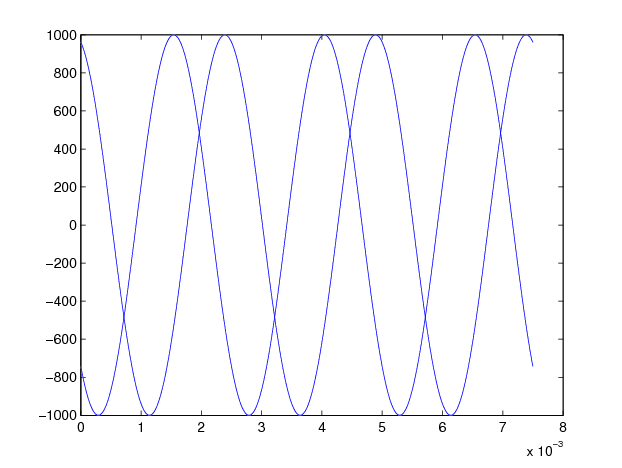
\includegraphics{2a.png}
	\caption{Plot twee ontvangen signalen}
	\end{center}
 \label{2a}
\end{wrapfigure}

\begin{wrapfigure}{r}{40mm}
	\begin{center}
	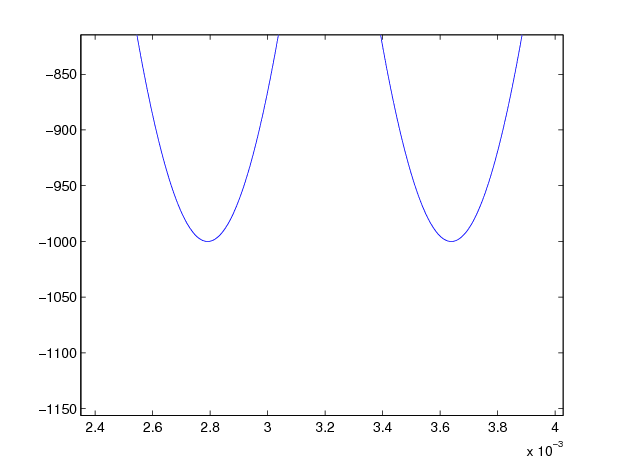
\includegraphics{2b.png}
	\caption{Plot ingezoomd op de dalen van de twee signalen}
	\end{center}
 \label{2b}
\end{wrapfigure}

\section{Opgave 3}
De waarde van \begin{math}\varphi\end{math} hebben we bepaald door middel van het tijdverschil van de twee ontvangen signalen, gegeven het verschil berekend in de vorige opgave, volgens:
$$\varphi = sin^{-1}(\frac{d}{c} * (t_{1} - t_{2})) = 0.79 rad$$

Tevens hebben we $\varphi$ berekend met behulp van de meetkunde. Dit geeft:
$$tan^{-1} (\frac{Xv}{Yr}) = 0.79rad$$

De gevonden waarde van $\varphi$ komen op twee significante cijfers overeen, dus de gebruikte methode blijkt te werken.

\section{Opgave 4}

De hoek tussen ontvanger en bron wordt berekend met de functie CalcDir. Deze functie verwacht twee complexe amplitudes die verkregen worden uit de geleverde functie DF\_Gen. De werking van de functie staat bij de code beschreven. 
\begin{lstlisting}
function [direction] = CalcDir(signal1, signal2)
%CALCDIR Calculates direction of the signals
%   given complex signals1 and 2, the direction is calculated by first
%   calculating de phase differences in rad. This is then converted to
%   seconds which is then used to calculate the direction. The direction is
%   returned in degrees.
    d = 0.4;
    ff = 400;
    ww = 2 * pi * ff;
    c = 1000/3;
    
    dfi = angle(signal1 .* conj(signal2));
    dt = dfi / ww;
    direction = real(asin(c/d*dt) * (180/pi));
end
\end{lstlisting}

Om het verschil in fase tussen de twee signalen te berekenen hebben we gebruik gemaakt van het feit dat $\Delta\varphi = angle\{X_{1}X_{2}^{*}\}$. Het bijbehorende bewijs staat hieronder gegeven.

$$X_{1} = A_{1}*e^{j\varphi_{1}}$$
$$X_{2} = A_{2}*e^{j\varphi_{2}}$$
$$angle\{X_{1}X_{2}^{*}\} = angle\{A_{1}*e^{j\varphi_{1}} * A_{2}*e^{-j\varphi_{2}}\}$$
$$= angle\{A_{1}*A_{2}*e^{j*(\varphi_{1}-\varphi_{2})}\}$$
$$= \varphi_{1}-\varphi_{2} = \Delta\varphi$$

\section{Opgave 5}
\begin{figure}
	\center
	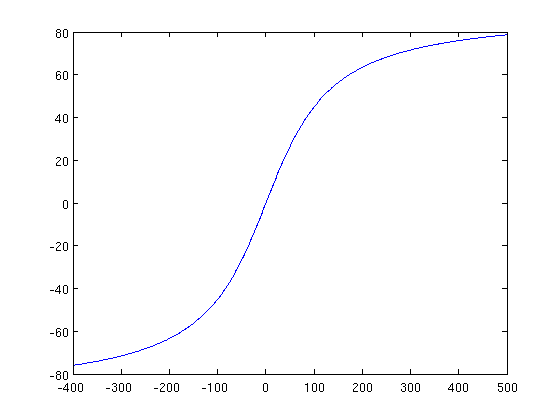
\includegraphics{5a.png}
	\caption{Plot gemaakt door functie TestDiff}
 \label{5a}
\end{figure}


In figuur \ref{5a}

\begin{figure}
 \label{5b}
\end{figure}

\end{document}